% Exam Template for UMTYMP and Math Department courses
%
% Using Philip Hirschhorn's exam.cls: http://www-math.mit.edu/~psh/#ExamCls
%
% run pdflatex on a finished exam at least three times to do the grading table on front page.
%
%%%%%%%%%%%%%%%%%%%%%%%%%%%%%%%%%%%%%%%%%%%%%%%%%%%%%%%%%%%%%%%%%%%%%%%%%%%%%%%%%%%%%%%%%%%%%%

% These lines can probably stay unchanged, although you can remove the last
% two packages if you're not making pictures with tikz.
\documentclass[11pt]{exam}
\RequirePackage{amssymb, amsfonts, amsmath, latexsym, verbatim, xspace, setspace, color, graphicx}


% By default LaTeX uses large margins.  This doesn't work well on exams; problems
% end up in the "middle" of the page, reducing the amount of space for students
% to work on them.
\usepackage[margin=1in]{geometry}
\usepackage[english]{babel}
\usepackage[autostyle]{csquotes} %%%% This package allows Tex to recognize quotation marks with the \enquote command. 


% Here's where you edit the Class, Exam, Date, etc.
\newcommand{\class}{MAT 203}
\newcommand{\term}{Summer I 2020}
\newcommand{\examnum}{Midterm}
\newcommand{\examdate}{06/11/20}
\newcommand{\timelimit}{3 hours and 25 minutes}

% For an exam, single spacing is most appropriate
\singlespacing
% \onehalfspacing
% \doublespacing

% For an exam, we generally want to turn off paragraph indentation
\parindent 0ex
\title{MAT 203 - Summer II 2020: Midterm solutions}
\begin{document} 

% These commands set up the running header on the top of the exam pages
\pagestyle{head}
\firstpageheader{}{}{}\textbf{}
\runningheader{\class}{\examnum\ - Page \thepage\ of \numpages}{\examdate}
\runningheadrule

\begin{flushright}
\begin{tabular}{p{2.8in} r l}
\textbf{\class} & \textbf{Name (Print):} & \makebox[2in]{\hrulefill}\\
\textbf{\term} &&\\
\textbf{\examnum} &&\\
\textbf{\examdate} &&\\
\textbf{Time Limit: \timelimit} & ID number & \makebox[2in]{\hrulefill}
\end{tabular}\\
\end{flushright}
\rule[1ex]{\textwidth}{.1pt}

\begin{center}
\large{\textbf{Instructions}}
\end{center}

\begin{minipage}[t]{3.7in}
\vspace{0pt}
\begin{itemize}

\item This exam contains \numpages\ pages (including this cover page) and
\numquestions\ problems.  Check to see if any pages are missing.  Enter
all requested information on the top of this page, and put your initials
on the top of every page, in case the pages become separated.

\item You may \textit{not} use your books, notes, or any device that is capable of accessing the internet on this exam (e.g., smartphones, smartwatches, tablets). You may use a calculator.

\item \textbf{Organize your work}, in a reasonably neat and coherent way, in
the space provided. Work scattered all over the page without a clear ordering will 
receive very little credit.  

\item \textbf{Mysterious or unsupported answers will not receive full
credit}.

\end{itemize}

\end{minipage}
\hfill
\begin{minipage}[t]{2.3in}
\vspace{0pt}
%\cellwidth{3em}
\gradetablestretch{2}
\vqword{Problem}
\addpoints % required here by exam.cls, even though questions haven't started yet.	
\gradetable[v]%[pages]  % Use [pages] to have grading table by page instead of question

\end{minipage}
\newpage % End of cover page

%%%%%%%%%%%%%%%%%%%%%%%%%%%%%%%%%%%%%%%%%%%%%%%%%%%%%%%%%%%%%%%%%%%%%%%%%%%%%%%%%%%%%
%
% See http://www-math.mit.edu/~psh/#ExamCls for full documentation, but the questions
% below give an idea of how to write questions [with parts] and have the points
% tracked automatically on the cover page.
%
%
%%%%%%%%%%%%%%%%%%%%%%%%%%%%%%%%%%%%%%%%%%%%%%%%%%%%%%%%%%%%%%%%%%%%%%%%%%%%%%%%%%%%%

\begin{questions}

% Basic question
%%%%%%%%%%%%%%

\addpoints
\question A heated storage room is to be constructed in the shape of a rectangular prism, with total volume $1000 \mathrm{ft}^3$. Because warm air rises, the heat loss per unit of area through the ceiling is five times as great as the heat loss through the floor. The heat loss through each of the four lateral walls is identical, equal to three times as much as the heat loss of the floor. 
\begin{parts}
\part[3] Sketch the room, labeling the dimensions of its sides. Describe the heat loss function according to your sketch. 

\textit{Solution:} Below is a sketch of the room.
\begin{center}
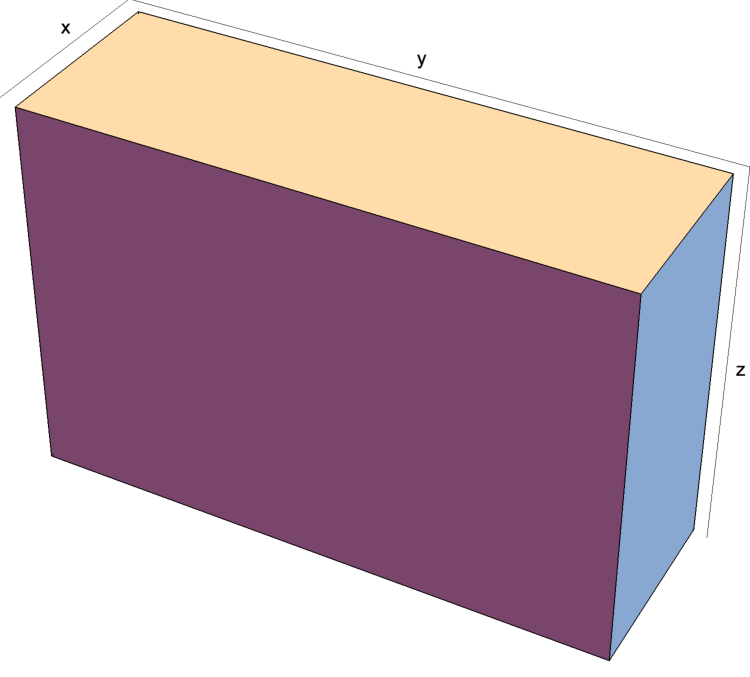
\includegraphics[scale=0.5]{p4.pdf}
\end{center}
Assume the heat loss through the floor is proportional to its surface area, $kxy$, for some positive constant $k$. Then the corresponding heat loss through the ceiling and lateral walls are $5kxy$, $3kyz$, $3kxz$. The total heat loss function is 
\begin{equation*}
f(x,y,z) = 6kxy + 6kyz + 6kxz
\end{equation*}
\vfill
\part[3] Use the volume constraint to reduce the number of variables in the heat loss function to two. 

\textit{Solution:} The volume constraint is $xyz=1000$. We can use it to eliminate $z$ in the heat loss function, 
\begin{equation*}
f(x,y) = 6kxy + \frac{6000k}{x} + \frac{6000k}{y}
\end{equation*}
\vfill
\part[4] Compute the gradient of the symplified heat loss function found on part (b). 

\textit{Solution:} The gradient is 
\begin{equation*}
\nabla f (x,y) = \left(6k y-\frac{6000k}{x^2},6kx-\frac{6000k}{y^2}\right).
\end{equation*}
\vfill
\newpage
\part[5] Find the critical points of the heat loss function. 

\textit{Solution:} Setting the coordinates of the gradient to $0$ leads to 
\begin{align*}
y & = \frac{1000}{x^2} \\
x & = \frac{1000}{y^2},
\end{align*}
a system whose only real solution is $x=10, y=10$.
\vfill
\part[5] Use the Second Partials Test to determine which critical point, if any, minimizes heat loss. 

\textit{Solution:} The Hessian of the heat loss function is 
\begin{equation*}
\mathrm{Hess} f (x,y)  = 
\begin{vmatrix}
\frac{12000k}{x^3} & 6k \\
6k & \frac{12000k}{y^3}
\end{vmatrix}.
\end{equation*}
At the critical point $(10,10)$, it becomes 
\begin{equation*}
\mathrm{Hess} f (10,10)  = 
\begin{vmatrix}
12k & 6k \\
6k & 12k
\end{vmatrix}.
\end{equation*}
Its determinant is $108k$, its trace is $24k$, both positive numbers, hence this critical point is a minimum. The dimensions of the room which minimizes heat loss under these circumstances are $x=10, y=10, z=10$.
\vfill
\end{parts}

\newpage 

%%%%%%%%%%%%%%%%%%%%%%%%%%%%%%%%%%%
\addpoints 
\question The table below shows the yield of a chemical reaction (measured in miligrams) in terms of time (measured in minutes):
\begin{center}
\begin{tabular}{|c|c|c|c|c|c|}
\hline 
Time & 1 & 2 & 3 & 4 & 5 \\ 
\hline 
Yield & 1.2 & 7.1 & 9.9 & 13.1 & 15.5 \\ 
\hline 
\end{tabular} 
\end{center}

\begin{parts}
\part[5] Given a line with equation $y=ax+b$, describe a function, in terms of the variables $a$ and $b$, measuring the sum of the square-distances between the points in the table above and the points with corresponding $x$-coordinate on the line.

\textit{Solution:} The coordinates of the corresponding points on the line are outlined in the table below. 
\begin{center}
\begin{tabular}{|c|c|c|c|c|c|}
\hline 
Time & 1 & 2 & 3 & 4 & 5 \\ 
\hline 
Yield & $a+b$ & $2a+b$ & $3a+b$ & $4a+b$ & $5a+b$ \\ 
\hline 
\end{tabular} 
\end{center}
The function that measures the sum of square-distances between the data set and the corresponding points on the line is 
\begin{align*}
f(a,b) & = (a+b-1.2)^2+(2a+b-7.1)^2+(3a+b-9.9)^2 \\
&  \, \, \, \, +(4a+b-13.1)^2+(5a+b-15.5)^2\\
& = 55 a^2+30 a b-350 a+5 b^2-93.6 b+561.72
\end{align*}
\vfill
\part[5] Find the gradient of the function you described in part (a). 

\textit{Solution:} The partial derivatives of $f$ are 
\begin{align*}
\partial_a f & = 110 a+30 b-350 \\
\partial_b f & = 30 a+10 b-93.6,
\end{align*}
hence the gradient is 
\begin{equation*}
\nabla f (a,b) = (110 a+30 b-350)\mathbf{i}+ (30 a+10 b-93.6)\mathbf{j}
\end{equation*}
\vfill
\newpage
\part[5] Find the critical points of the function you described in part (a).

\textit{Solution:} The critical points are found by setting the coordinates of the gradient to zero,
\begin{align*}
110 a+30 b-350 & = 0,\\
30 a+10 b-93.6 & = 0.
\end{align*}
A solution to this system may be found by elimination. For instance, subtracting three times the second equation from the first yields
\begin{equation*}
20a = 69.2 \Rightarrow a = 3.46,
\end{equation*}
and by substitution into either of the two equations we find $b = -1.02$.
\vfill
\part[5] Find the equation of the regression line approximating the points in the table by determining which of the critical points you found on part (c), is a minimum. 

\textit{Solution:} There is only one critical point, so all we need to do is to confirm it is a minimum via the Second Partials Test. The Hessian of the function $f$ is 
\begin{equation*}
\begin{vmatrix}
110 & 30 \\
30 & 10
\end{vmatrix}.
\end{equation*}
Its determinant at $(a,b) = (3.46, -1.02)$ is $200$ and its trace is $120$, both positive numbers, hence the critical point is a local minimum. This being the only critical point, it must be in fact a global minimum, therefore confirming that the regression line is given by the equation
\begin{equation*}
y = 3.46x-10.2
\end{equation*}
\vfill
\end{parts}

\newpage

%%%%%%%%%%%%%%%%%
\addpoints
\addpoints
\question This problem concerns the iterated integral
\begin{equation*}
\int_{0}^{4} \int_{\sqrt{x}}^{2} \frac{3}{2+y^3} \, dy \, dx.
\end{equation*}

\begin{parts}
\part[5] Sketch the region of integration in the plane.

\textit{Solution:} A plot of the region of integration is represented below. 
\vspace{1cm}
\begin{center}
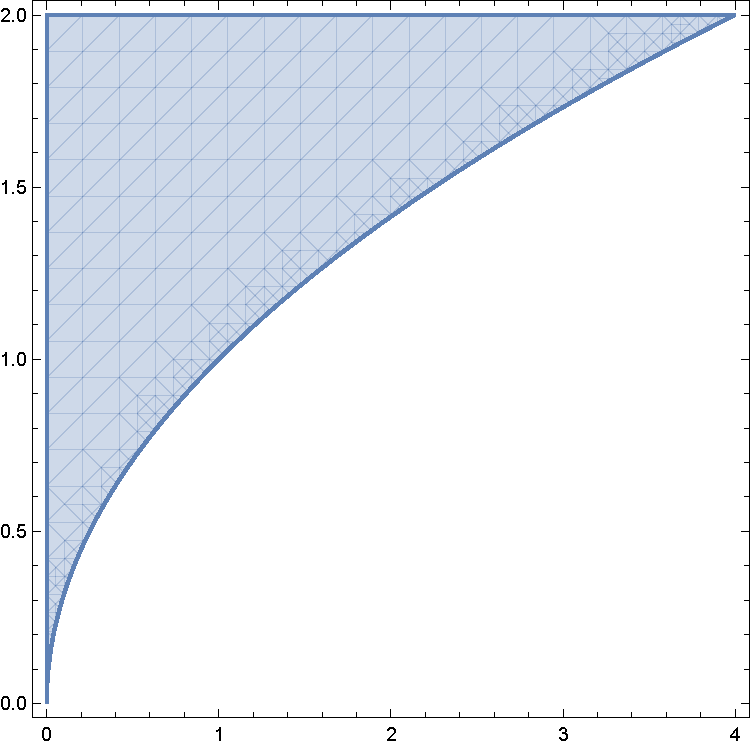
\includegraphics[scale=0.5]{p2.pdf}
\end{center}
\vfill 
\part[5] Switch the order of integration.

\textit{Solution:} 
\begin{equation*}
\int_{0}^{2} \int_{0}^{y^2} \frac{3}{2+y^3}\, dx \, dy
\end{equation*}
\vfill
\newpage
\part[10] Evaluate the integral by using whichever order you prefer. 

\textit{Solution:} The simpler order of integration is the one from part (b). In this order, the integral can be evaluated as
\begin{align*}
\int_{0}^{2} \int_{0}^{y^2}  \frac{3}{2+y^3}\, dx \, dy & = \int_{0}^{2} \left[ \frac{3x}{2+y^3} \Big|_{x=0}^{x=y^2} \right] \, dy \\
& = \int_{0}^{2}  \frac{3y^2}{2+y^3} \, dy \\
& = \left[ \log(2+y^3)\Big|_{y=0}^{y=2} \right] \\
& = \log(10)-\log(2) \\
& = \log(5)
\end{align*}
where in the third step we used the substitution $u=2+y^3$. 
\vfill
\end{parts}

\newpage
%%%%%%%%%%%%%%%%%

\addpoints
\question[10] Use polar coordinates to find the area between outside of the circle of radius 1 and inside the cardioid with equation 
\begin{equation*}
r = 2+ \cos(\theta)
\end{equation*}

\textit{Solution:} This area may be computed by means of the following integral
\begin{align*}
\int_{0}^{2\pi} \int_{1}^{2+\cos(\theta)} r \, dr \, d\theta & = \int_{0}^{2\pi} \left[ \frac{r^2}{2} \Big|_{r=1}^{r=2+\cos(\theta)} \right] \, d\theta \\
& = \int_{0}^{2\pi} \frac{(2+\cos(\theta))^2}{2} - \frac{1}{2} \, d\theta \\
& = \int_{0}^{2\pi} \frac{3}{2}+2\cos(\theta)+\frac{\cos^2(\theta)}{2} \, d\theta \\
& = \int_{0}^{2\pi} \frac{3}{2}+2\cos(\theta)+ \left(\frac{\cos(2\theta)+1}{4}\right) \, d\theta \\
& = \frac{7\pi}{2},
\end{align*}
since the trigonometric functions integrated over the range $(0,2\pi)$ yield $0$ as a result. 
\newpage

%%%%%%%%%%%%%%%%%%%%
\addpoints
\question This problem concerns the iterated integral
\begin{equation*}
\int_{-1}^{1} \int_{-\sqrt{1-x^2}}^{\sqrt{1-x^2}} \int_{1}^{1+\sqrt{1-x^2-y^2}} x \, dz \, dy \, dx.
\end{equation*}
Below is a plot of the region of integration, for your convenience.
\begin{center}
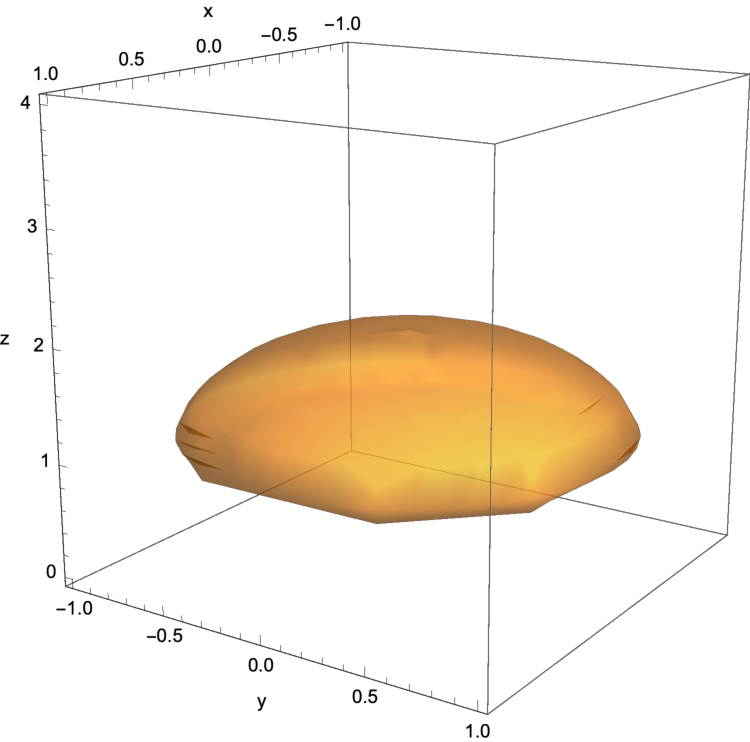
\includegraphics[scale=0.5]{p1.pdf}
\end{center}
\begin{parts}
\part[8] Convert it to cylindrical coordinates (do not evaluate).

\textit{Solution:} The ranges for the axial radius and polar angle are simpler: $[0,1]$, and $[0,2\pi]$, respectively. The range of values for the height function $z$ can be stated in terms of cylindrical coordinates as
\begin{equation*}
[1,1+\sqrt{1-x^2-y^2}] = [1,1+\sqrt{1-r^2}].
\end{equation*}
The integral is expressed in terms of cylindrical coordinates as 
\begin{equation*}
\int_{0}^{2\pi} \int_{0}^{1} \int_{1}^{1+\sqrt{1-r^2}} r^2\cos(\theta) \, dz \, dr \, d\theta.
\end{equation*}
\vfill
\newpage
\part[8] Convert it to spherical coordinates (do not evaluate).

\textit{Solution:} The simpler spherical variable is the longitude angle, which ranges from $0$ to $2\pi$. We will choose it as the independent variable.

We will choose the latitude angle $\phi$ (measured from the North Pole) as the next variable in line for integration. Clearly the lowest variable it can take is $0$ (this happens for all points along the $z$ axis). Notice that the upper limit of integration does not depend on the longitude angle, as the curve at the intersection between the upper and lower surfaces bounding this region of integration is rotationally symmetric about the $z$-axis. at this intersection, $z=1$, and in addition
\begin{equation*}
1+\sqrt{1-x^2-y^2}=1 \Rightarrow x^2+y^2 =1.
\end{equation*}
The radius (measured as distance from the origin) at such points is
\begin{equation*}
r_{\mathrm{intersection}} = \sqrt{x^2+y^2+z^2} = \sqrt{1+1} = \sqrt{2}.
\end{equation*}
We can find the latitute angle at the intersection by means of the relation $z =r\cos(\phi)$, 
\begin{equation*}
1 = \sqrt{2} \cos(\phi_{\mathrm{upper}}) \Rightarrow \phi_{\mathrm{upper}} = \frac{\pi}{4}.
\end{equation*}

Next is the range of radii. In this case, both the upper and lower bounds depend on the latitude angle. Below is a projection of the region of integration on the $yz$-plane, used for reference in subsequent calculations.

\begin{center}
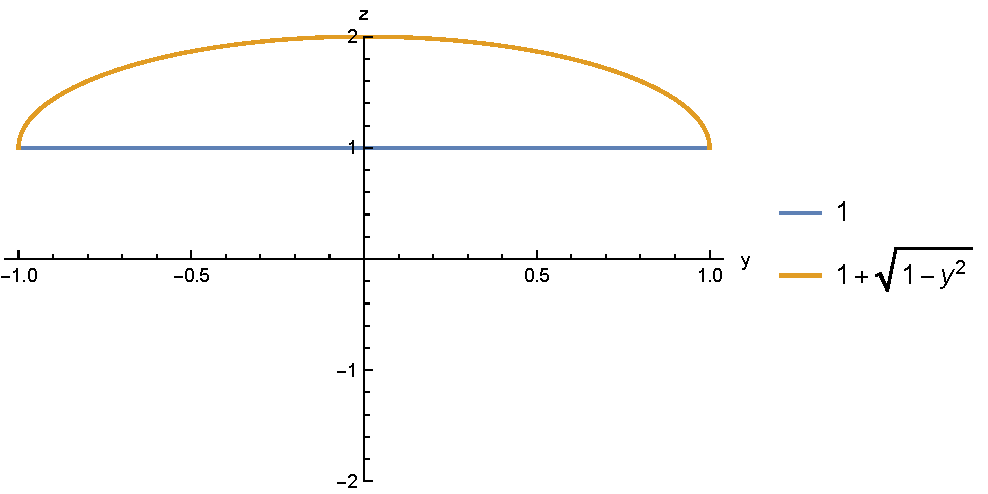
\includegraphics[scale=0.5]{p3.pdf}
\end{center}

The value of $z$ at altitude $1$ is related to $r_{\mathrm{lower}}$ by 
\begin{equation*}
r_{\mathrm{lower}}\cos(\phi) = 1 \Rightarrow r_{\mathrm{lower}} = \sec(\phi)
\end{equation*}
The corresponding value of $z$ at altitude $1+\sqrt{1-y^2}$ is related to $r_{\mathrm{upper}}$ and $\phi$ by 
\begin{equation*}
r_{\mathrm{upper}}\cos(\phi) = 1+ \sqrt{1-r_{\mathrm{upper}}^{2}\sin^{2}(\phi)}.
\end{equation*}
By rearranging terms and squaring, we obtain
\begin{align*}
r_{\mathrm{upper}}\cos(\phi) -1 & = \sqrt{1-r_{\mathrm{upper}}^{2}\sin^{2}(\phi)} \\
r_{\mathrm{upper}}^2\cos^2(\phi)-2r_{\mathrm{upper}}\cos(\phi)+1 &= 1-r_{\mathrm{upper}}^{2}\sin^{2}(\phi) \\
r_{\mathrm{upper}}^2\cos^2(\phi) + r_{\mathrm{upper}}^{2}\sin^{2}(\phi) & = 2r_{\mathrm{upper}}\cos(\phi) \\
r_{\mathrm{upper}} = 2\cos(\phi).
\end{align*}

The integral can therefore be written in spherical coordinates as 
\begin{equation*}
\int_{0}^{2\pi} \int_{0}^{\frac{\pi}{4}} \int_{\sec(\phi)}^{2\cos(\phi)} r^3\sin^2(\phi)\cos(\theta) \, dr \, d\phi \, d\theta
\end{equation*}
\vfill
\newpage
\part[14] Evaluate the integral by using your preferred system of coordinates: Cartesian, cylindrical, or spherical. 

\textit{Solution:} The integral can be evaluated in cylindrical coordinates by interchanging the order of integration,
\begin{align*}
\int_{0}^{2\pi} \int_{0}^{1} \int_{1}^{1+\sqrt{1-r^2}} r^2\cos(\theta) \, dz \, dr \, d\theta & = \int_{0}^{1} \int_{1}^{1+\sqrt{1-r^2}} \int_{0}^{2\pi}  r^2\cos(\theta) \, d\theta \, dz \, dr  \\
& = \int_{0}^{1} \int_{1}^{1+\sqrt{1-r^2}} r^2\sin(\theta) \Big|_{\theta = 0}^{\theta = 2\pi} \, dz \,dr \\
& = \int_{0}^{1} \int_{1}^{1+\sqrt{1-r^2}} 0 \, dz \,dr \\
& = 0.
\end{align*}

Think about it: could you have predicted the outcome based solely on the plot provided?
\vfill
\end{parts}


%%%%%%%%%%%%%%%%%%%%%%%%%%

\end{questions}
\end{document}
